\textit{Cu.Te}, o ClUstering TrajectoriEs, è un algoritmo di clustering overlapping il cui obbiettivo è l'analisi
di gruppi di oggetti in movimento. Questa ricerca viene condotta considerando sia la dimensione spazio-temporale
delle traiettorie sia eventuali dimensioni semantiche (come ad esempio, le municipalità di una città).

Lo scenario reale per la realizzazione di questo algoritmo è stata l'analisi condotta su
un insieme di traiettorie generate a Milano. All'interno di questo studio, i pattern di movimento sono
stati analizzati a diversi livelli.
Una prima analisi è stata condotta dividendo la superfice della città in piccole celle:questa ricerca
ha rivelato i pattern di movimento del traffico, individuando quali potessero essere le strade
maggiormente frequentate.
Succesivamente è stato realizzato uno studio basato sul vicinato: questo ha individuato i flussi di spostamento per specifiche categorie di utenti.
Infine una ricerca basata sulle municipalità ha mostrato quali fossero le aree della città più visitate da differenti gruppi di individui.

Lo scopo di \textit{Cu.Te} è dunque di estrarre i pattern di movimento che avvengono con una certa soglia di frequenza.

L'algoritmo \textit{Cu.Te} è etichettabile come algoritmo di \textit{colossal trajectory mining}.
L'idea alla base del \textit{colossal trajectory mining},
o mining di traiettorie su larga scala, interseca entrambi gli ambiti del clustering di traiettorie
e del \textit{colossal itemset mining}.


Il \textit{colossal itemset mining} si pone come un'estensione del \textit{frequent itemset mining}
presentato nella~\cref{sec:problem:frequent-itemset-mining}. Questa espansione riguarda l'utilizzo di dati
a elevata dimensionalità~\cite{zhu2007mining}, in alcuni domini è possibile infatti che il numero di attributi per ogni dato sia di molto superiore al numero stesso di dati.
Tale prospettiva può essere impiegata anche nell'analisi di dati di traiettoria. Considerando la superfice
spazio-temporale coperta dall'insieme delle traiettorie e il numero di queste ultime, nella maggior parte dei casi risulterà evidente
che la dimensionalità di quest'ultimo dato sarà maggiore del precedente.

Risulta quindi possibile applicare algoritmi di mining di itemset su larga scala a dati di traiettoria.
In letteratura è possibile trovare riferimenti ad algoritmi di \textit{colossal itemset mining}~\cite{DBLP:journals/bdr/ApilettiBCGPM17, DBLP:conf/kdd/PanCTYZ03}
, tuttavia nessuno di questi è adatto alla ricerca di pattern di movimento, anche per la mancanza di
criteri di pruning basati sulle dimensioni spazio-temporali. Nonostante quindi la letteratura non
presenti una soluzione adatta, le idee alla base del \textit{colossal itemset mining} risultano sicuramente interessanti.

Parlando poi di clustering di traiettorie, rispetto a quanto trattato nella nella~\cref{sec:problem:trajectoryclustering}, è possibile aggiungere un'ulteriore divisione:
si definisce il clustering partizionante se ogni punto appartiene a un solo cluster, sovrapposto in caso contrario.
Applicando questo principio di classificazione agli algoritmi basati su traiettorie, gli algoritmi partizionanti considereranno la traiettoria nella sua interezza,
assegnandola quindi ad un solo cluster. Questa tipologia di clustering comporta però la perdita di informazioni tra i diversi cluster:
nonostante una traiettoria sia raggruppata in un cluster che massimizza la similarità tra i propri elementi,
questa può comunque condividere pattern interessanti con altre traiettorie appartenenti a cluster differenti.

Per superare il problema descritto sopra, gli algoritmi di clustering sovrapposto effettuano una divisione di ogni traiettoria
in sotto-traiettorie e effettuano un clustering partizionante su queste sotto-traiettorie.
Questa soluzione permette di conservare le relazioni intra-cluster, tuttavia una frammentazione troppo fine può causare
la perdita di \textit{rare pattern}, ad esempio eventi significanti che accadono con una bassa frequenza~\cite{DBLP:journals/tkdd/KohR16, DBLP:journals/geoinformatica/HuangPX06}.

Come già detto nella~\cref{sec:problem:trajectoryclustering}, il clustering classico non esprime vincoli temporali o ulteriori parametri adatti alla ricerca di traiettorie.
Per aggiungere la possibilità di esprimere vincoli sul tempo, sono stati introdotto i \textit{co-movement} patterns descritti nella~\cref{sec:problem:comovements-pattern}; algoritmi come \textit{G.C.M.P},
(~\cref{chapter:chapter2}), \textit{GeT Move}~\cite{DBLP:journals/ijitdm/PhanPT16} e  implementa la ricerca di questi pattern mischiando l'approccio basato su \textit{frequent itemset mining} e il clustering.
Entrambi questi framework discretizzano il tempo in bucket di dimensione finita, su cui poi applicano un clustering basato sulla densità, infine
ricercano pattern di movimento fondendo i vari cluster ottenuti nei differenti istanti temporali.

Rispetto a quanto presentato fin d'ora, \textit{Cu.Te} presenta le seguenti caratteristiche:

\begin{itemize}

  \item Flessibilità nell'impiego di dimensioni: all'interno di \textit{Cu.Te} è possibile aggiungere
  dimensioni personalizzate su cui condurre la ricerca, ad esempio si può espandere la dimensione spazio
  temporale aggiunendo il concetto di municipalità.
  Inoltre sono supportate dimensioni non esclusivamente monotone, come ad esempio i giorni della settimana.

  \item Continuità nello spazio tempo: nella ricerca di \textit{comomvement pattern} è possibile specificare vincoli di contiuità non solo sul tempo, ma anche sullo spazio.

  \item Efficienza nel pruning spazio-temporale: la strategia di pruning impiegata permette di ridurre
  lo spazio di ricerca dell'algoritmo sulla base della natura spazio-temporale delle traiettorie.

  \item Efficacia rispetto a problemi reali: \textit{Cu.Te} mette a disposizione una soluzione distribuita per il problema del \textit{Colossal Trajectory Mining}
  compatibile con dataset costruiti su problemi del mondo reale.
\end{itemize}


L'algoritmo segue tre step per la formazione dei cluster, come anche rappresentato in~\cref{fig:chap-3:cute-overview}

  \begin{figure}
    \centering
    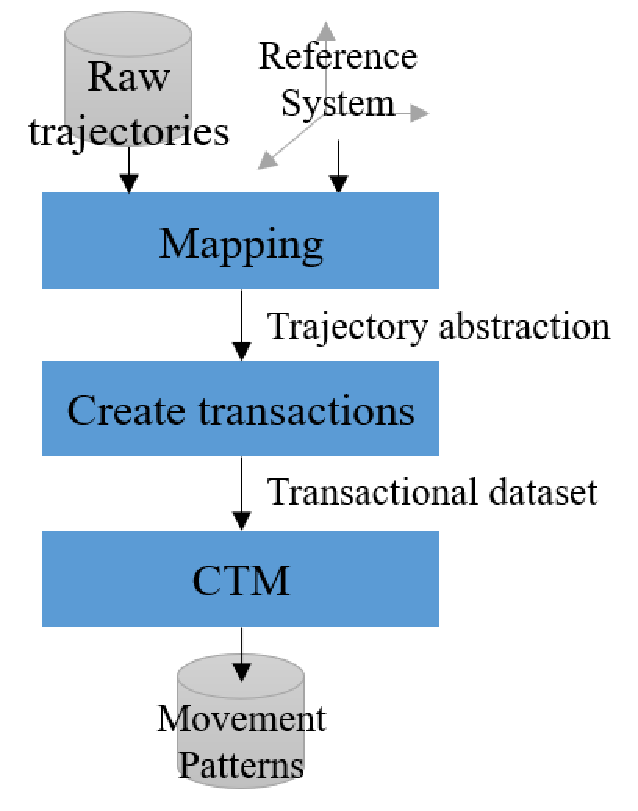
\includegraphics{/sec-3/cute-algorithm-overview.pdf}
    \caption{Rappresentazione grafica delle tre fasi dell'algoritmo Cu.Te,Fonte:~\url{https://which.souce?}}%
    \label{fig:chap-3:cute-overview}
  \end{figure}

  \begin{enumerate}
    \item \textbf{Mapping delle traiettorie:}

    In questo primo passo vengono analizzate le traiettorie presenti nel dataset. Da queste viene determinata la regione spazio-temporale
    in cui tutti gli oggetti si sono mossi. Successivamente l'area di movimento viene divisa in un insieme di celle omogenee per dimensioni nello spazio e nel tempo.
    A questo punto ad ogni traiettoria viene assegnato un insieme di celle secondo il seguente principio: una cella è attribuita ad una traiettoria quando quest'ultima ha
    almeno un punto che ricade entro i confini spazio-temporali della cella.

    \item  \textbf{Creazione delle transazioni:}

    Durante questa fase vengono poste le basi per l'\textit{itemset mining}: scopo di questa parte dell'algoritmo
    è infatti andare a generare l'insieme delle transazioni su cui verrà eseguita la ricerca di pattern.
    Ciò avviene considerando l'ouput della fase precedente e ribaltando la relazione cella traiettoria:
    mentre prima le traiettorie venivano condiderate in termini di celle percorse, ora si considera ogni cella in relazione alle traiettorie che almeno per
    un istante transitano al suo interno.

    \item \textbf{Colossal Trajectory Mining:}

    Ultima e più importante passaggio dell'algoritmo, produce in uscita i pattern di movimento.
    Dato l'output della fase precedente, ovvero un insieme di transazioni appositamemte creato,
    esegue una ricerca di itemset su dati ad alta dimensionalità.

  \end{enumerate}





